\documentclass[../../Aurora C# unofficial manual.tex]{subfiles}

\begin{document}
	\section{Ground formation element transfer UI}\label{ground_formation_element_transfer_ui}
	Original post can be found
	\href{http://aurora2.pentarch.org/index.php?topic=8495.msg109808#msg109808}{here}.
	\\\\
	
	Below is the same screenshot as the previous post but with the Elements option selected. Now the formation elements for each Ground Formation are shown in the hierarchy. For formations with no subordinate formations, the formation elements are shown directly under the parent formation. For formations with subordinate formations, the formation elements are shown under their own node, to avoid cluttering the tree view.
	
	To move elements between formations, you can drag and drop elements from one formation to another, although they must be on the same system body. Normally, the whole element is transferred. However, if the Amount checkbox is checked, a popup box will appear after the drag-drop, allowing you to transfer only a portion of the element. If the receiving formation already has an element with the same ground unit class, the additional units will be added to the existing element.
	\begin{figure}[H]
		\centering
		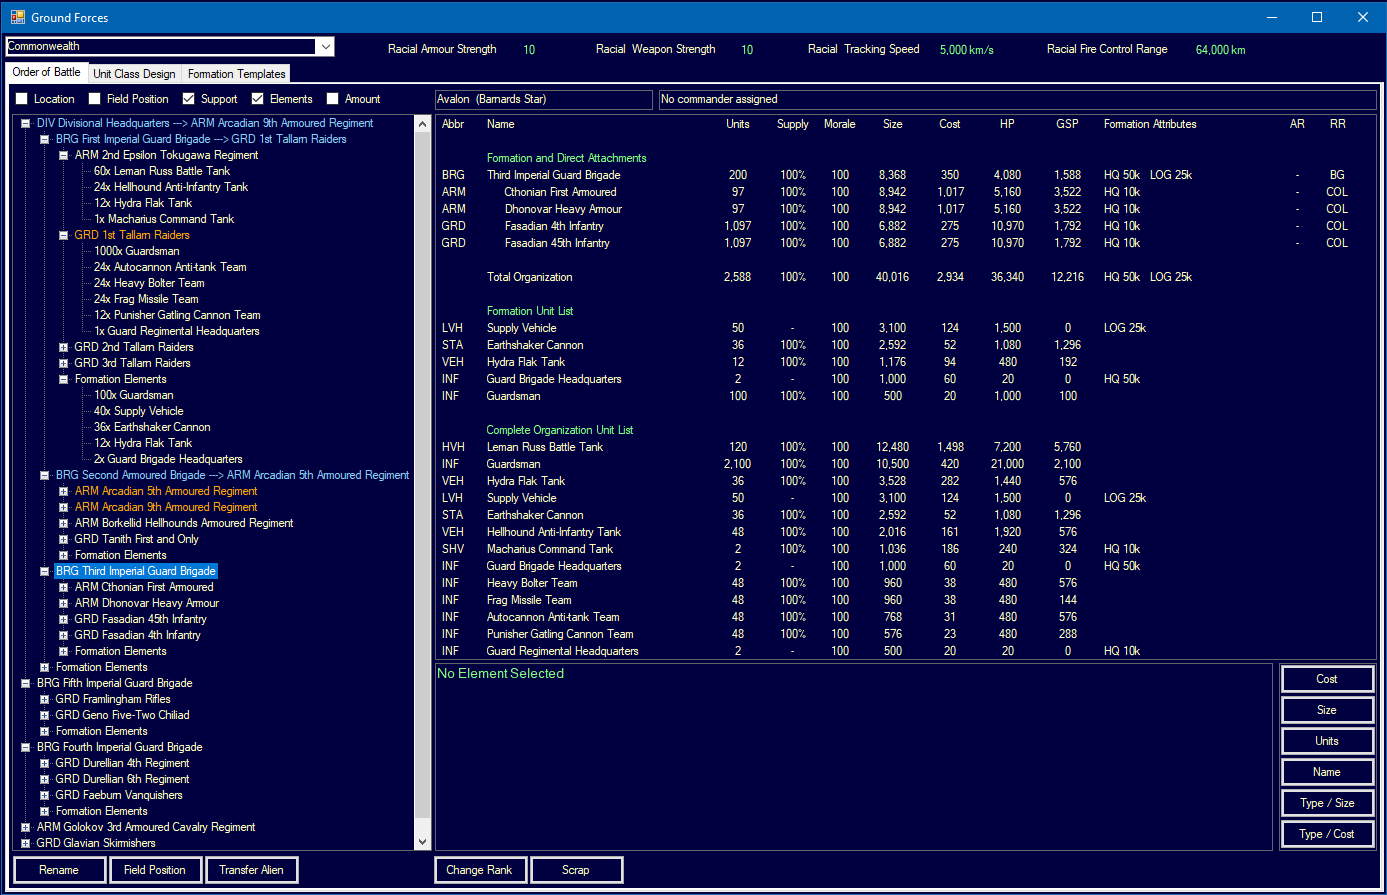
\includegraphics[width=0.9\linewidth]{images/ElementsUI}
		\caption[Elements UI]{Formation transfer UI}
		\label{fig:elementsui}
	\end{figure}
\end{document}